\section{System- und Kontextgrenze} \label{SystemKontextGrenze}

Über die System- und Kontextgrenzen wird der Rahmen für das Projekt gesetzt. Man unterscheidet zwischen System (\textit{kann beeinflusst werden}), Systemkontext (\textit{ist relevant für das Projekt, jedoch können solche Aspekte nicht beeinflusst werden}) und irrelevanter Umgebung (\textit{spielt zum jetzigen Zeitpunkt keine Rolle}).

\begin{figure}[h!]
	\centering
	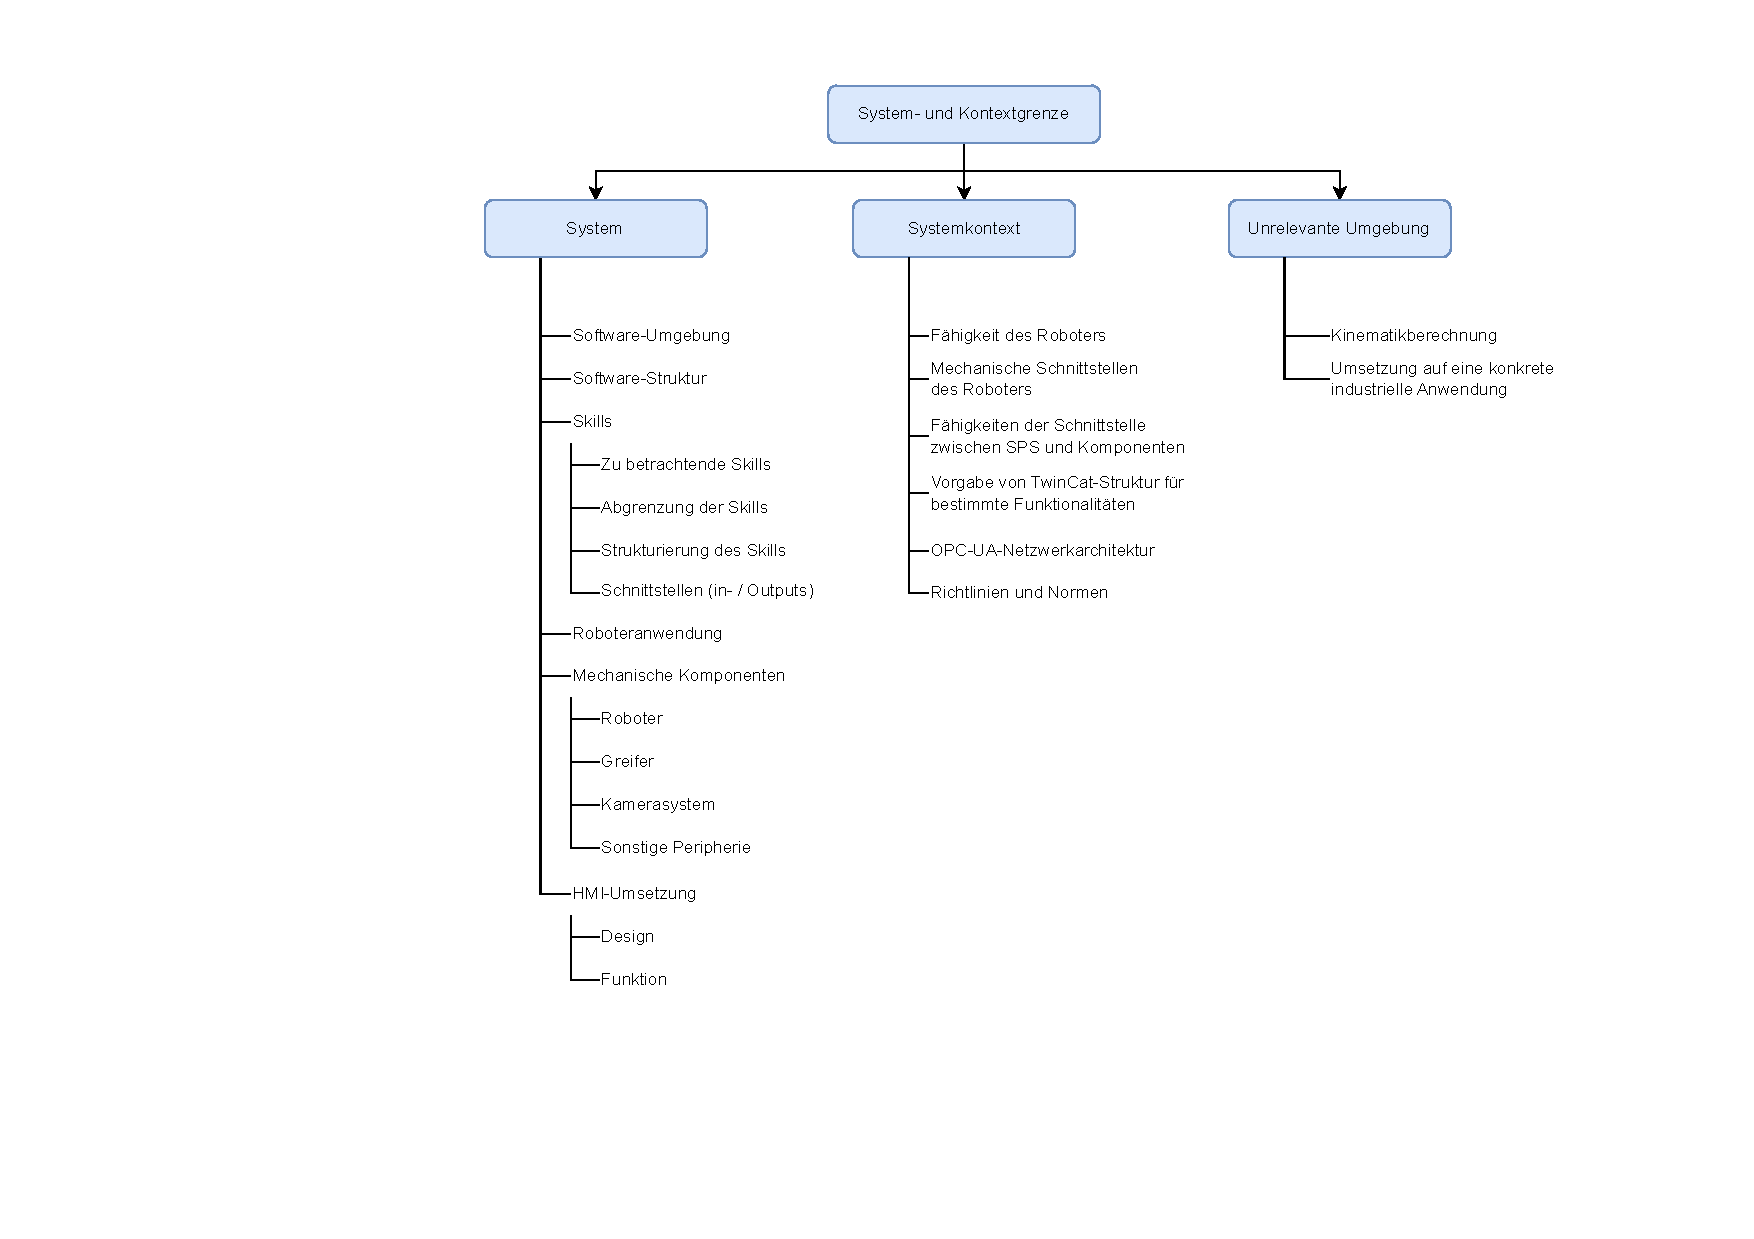
\includegraphics[width=1\textwidth]{02_Einfuehrung_in_Thematik/SystemKontextGrenze}
	\captionsetup{justification=centering}
	\caption{System- und Kontextgrenzen}
	\label{fig:SystemKontextGrenze}
\end{figure}

\newpage